\chapter{Introduction}
%-------------------------------------------------------------------------------
\section{Presentation of the \stbtel software}
%-------------------------------------------------------------------------------
%
when a model is constructing with the \telemacsystem, the mesh computation is
an important step. Most of the time, this operation is done with the integrated
mesh generator MATISSSE; however, the \telemacsystem allows the interface with
some other mesh generator software. So, the aim of the \stbtel software is to
realise this interface within the \telemacsystem software. Moreover, it permits
also a lot of operations on these meshes:
\begin{itemize}
\item Check of the geometry
\item Interpolation of the bathymetric points
\item Dry elements elimination when using a \telemac{2D} results file
\item Mesh extraction
\end{itemize}
Mesh files of the following list are interfaced with the \stbtel version 4.1:
\begin{itemize}
\item The SIMAIL manufactured by SIMULOG.
\item The I-DEAS manufactured by SDRC
\item The TRIGRID program developed by the Institute of Ocean Sciences, Canada
\item The FASTTABS program developed by the Brigham Young University, USA
\end{itemize}
Of course, standard format file of the \telemacsystem (Selafin) can be used by
\stbtel.\\
\stbtel was developed by the National Hydraulics Laboratory (Laboratoire
National d’Hydraulique-LNH) of the Research and Studies Directorate of the
French Electricity Board (EDF-DER). Like previous versions of the program,
version 4.1 complies with EDF-DER’s Quality Assurance procedures for scientific
and technical programs. This sets out rules for developing and checking product
quality at all stages. In particular, a program covered by Quality Assurance
procedures is accompanied by a Formulation Document [01] that describes the
theoretical aspects of the software, and a Validation Document [02] that
describes the validation domain of the software and a set of test cases. This
latter document can be used to determine the performance and limitations of the
software and define its field of application. The test cases are also used for
developing the software and are checked each time new versions that are
produced.

%-------------------------------------------------------------------------------
\section{Situation of \stbtel software within the \telemacsystem modelling system}
%-------------------------------------------------------------------------------

The \stbtel software is part of a complete set of computational software and
their associated pre- and post-processors, the \telemacsystem. This offers all
the modules required for 2D and 3D numerical simulations in hydrodynamics
(currents and waves), sedimentology and water quality.\\
%
\begin{figure}[H]%
\begin{center}
%
  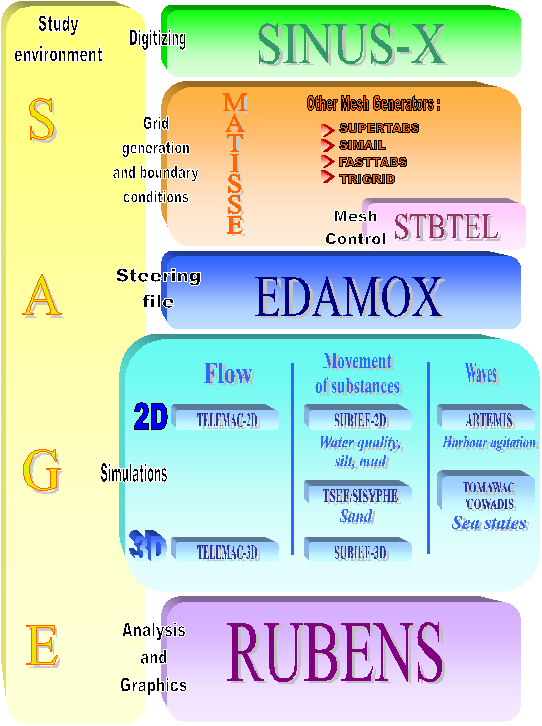
\includegraphics[width=0.9\textwidth]{./graphics/orga}
%
\end{center}
\caption
{Organisation of the modules.}
\label{fig:orga}
\end{figure}

The \telemacsystem, illustrated on figure \ref{fig:orga}, consists of the following
modules:
\begin{itemize}
\item The SINUSX [03] software. This is used, in conjunction with a digitising
pad, to acquire bed data and the limits of the domain that is to be simulated
with the model. The mesh generator will then read the corresponding file.
\item The MATISSE [04] software. This is used to build the grid based on
triangular elements, using the bathymetry.
\item The \stbtel software. This is used, reading the file produced by the mesh
generator, for interpolating bathymetric data (optionally) and creating a
geometry file to the Selafin standard that can be read by the simulation
modules and by the RUBENS graphical post-processor. \stbtel also carries out a
number of mesh consistency checks. Its use is described in this manual.
\item The \telemac{2D} [05] software. This carries out the hydrodynamic
simulation. \telemac{2D} is also able to simulate the transport of dissolved
tracers.
\item The EDAMOX [06] software. This enables interactive creation of the
steering files required for the various simulation modules.
\item The SUBIEF [07] software. This is used to simulate water quality
phenomena (calculation of the transport by advection/dispersion of dissolved
substances without buoyancy effects) and the transport of suspended sediments.
\item The \sisyphe [08] software. This is used to simulate the transport of bed
load (\sisyphe supersedes the TSEF software within the \telemacsystem)
\item The \artemis [09] software. This computes the transformation of wave
characteristics in a coastal area or harbour.
\item The \telemac{3D} [10] software which computes 3D hydrodynamics.
\telemac{3D} is also able to simulate the transport of dissolved tracers.
\item The \postel [11] software which produces 2D cuts inside the 3D results
file of \telemac{3D}, in order to use the RUBENS graphical post-processor.
\item The RUBENS [12] software. This is used for interactively exploiting and
producing graphical outputs of the results of the various simulation modules.
\item The SAGE software which offers help for the studies management.
\end{itemize}

%-------------------------------------------------------------------------------
\section{Computer environment}
%-------------------------------------------------------------------------------

The simulation modules are written in FORTRAN-77, with no machine-specific
language extensions. A shift to FORTRAN-90 is in progress. They can be run on
all workstations operating under UNIX and on certain vector computers (in
particular Cray and Fujitsu). At EDF-DER, these programs were developed on a
Cray vector computer operating under Unicos and on a HP 9000 series 700
workstation operating under HP-UX.\\
The graphics modules (SINUSX, RUBENS, EDAMOX and MATISSE) can be run on a
workstation operating under UNIX with access to X\_Windows X11R5 and OSF/Motif
libraries

